\documentclass[12pt]{article}

\usepackage{amsmath, amssymb, amsthm}
\usepackage{enumerate}
\usepackage{listings}
\usepackage{changepage}
\usepackage{pgfplots, pgfplotstable}

\title{CS325 Winter 2013: Implementation 2}
\author{
    Daniel Reichert \\
    Trevor Bramwell
}
\date{\today}

\begin{document}
\maketitle

\section{Theoretical Analysis}
\subsection{Pseudocode}
    The following is pseudocode to solve the Maximum Subarray problem.
\paragraph{}
Brute Force Pseudo:
    \begin{lstlisting}[basicstyle=\ttfamily\small,mathescape]

    brute_sum(n)
        size = the size of n
        max = first element in the n array
        for i = 0 .. size+1:
            sums = array of size+1 with each element initialized to n[0]
            for j = i+1 .. size+1:
                if i < j:
                    sums[j] = the sum of the elements from i to j-2 plus n[j-1]
                    if sums[j] > max_sum:
                        max = sums[j]
        return max

    \end{lstlisting}


\paragraph{}
Divide and Conquer Pseudo:
    \begin{lstlisting}[basicstyle=\ttfamily\small,mathescape]

    divide_conquer(n)
        # a miracle occurs
        return maximum contiguous subarray

    \end{lstlisting}
        

\paragraph{}
Dynamic Pseudo:
    \begin{lstlisting}[basicstyle=\ttfamily\small,mathescape]

    dynamic(n)
        cummulative = 0
        high_water = n[0]
        for i = 0 .. size of n
            cummulative = max of (0, cummulative+n[i])
            high_water = max of (cummulative, high_water)
        return high_water

    \end{lstlisting}

\section{Asymptotic Run Time Analysis}
    \begin{enumerate}

    \item In the brute force algorithm there are no subproblems.  With the
            nested for loops, there is a comparison made between every element
            in the input, leading to an intutitive asymptotic complexity of 
            $O(n^2)$

	\item In the divide and conquer algorithm the problem is branched into 
            $2$ subproblems for a size of $n/2$ at each level.  Those two
            subproblems cover the two cases where the maximal subsequence
            is fully contained within either half of the array.  The case
            where the maximal subsequence is contained partially in each
            half of the array can be analyzed in linear time.  Which leads
            to a complexity statement of $T(n) = 2T(n/2) + O(n)$.  Per the
            master theorem, this leads to a complexity of $O(n log n)$.

    \item In the dyanmic programming algorithm the problem is approached 
            from the bottom up. Like all dynamic programming algorithms
            the complexity can be modeled by the size of the table that is
            created multiplied by the time it takes to fill in a cell of that
            table.  Since the time to fill in a cell is constant and the table
            is 1 dimensional, the run time is $c*n$ or $O(n)$   
     \end{enumerate}

\section{Theoretical Correctness}
    \begin{enumerate}

    \item In the Divide and conquer algorithm the problem is divided into two
            halves.  The maximal subsequence can be contained in one of three
            different cases.  The first two cases are when the maximal
            subsequence is contained entirely in one of the two halves. The 
            third case is when the maximal subsequence is partially in both
            halves of the array.  Since the algorithm considers all three of
            these cases we know that the algorithm will calculate the correct
            maximum value.

    \item In the Dynamic programming algorithm every possible case is 
            considered in a linear fashion.  Since the maximum value of all
            cases that have been considered is continually updated with each
            new subsequence, we know that the maximum value will be captured.

    \end{enumerate}

\section*{Empirical Testing}

\begin{center}
\begin{tabular}{|c|c|}
\hline
verify.txt & test\_input.txt \\ \hline
9670  & 249310 \\ \hline
10567 & 252709 \\ \hline 
9282  & 253719 \\ \hline 
9269  & 249315 \\ \hline 
9675  & 247789 \\ \hline 
10378 & 254833 \\ \hline 
9911  & 239844 \\ \hline 
9790  & 257527 \\ \hline 
9580  & 241669 \\ \hline 
9965  & 255628 \\
\hline
\end{tabular}
\end{center}

\section*{Empirical Analysis of Runtime}

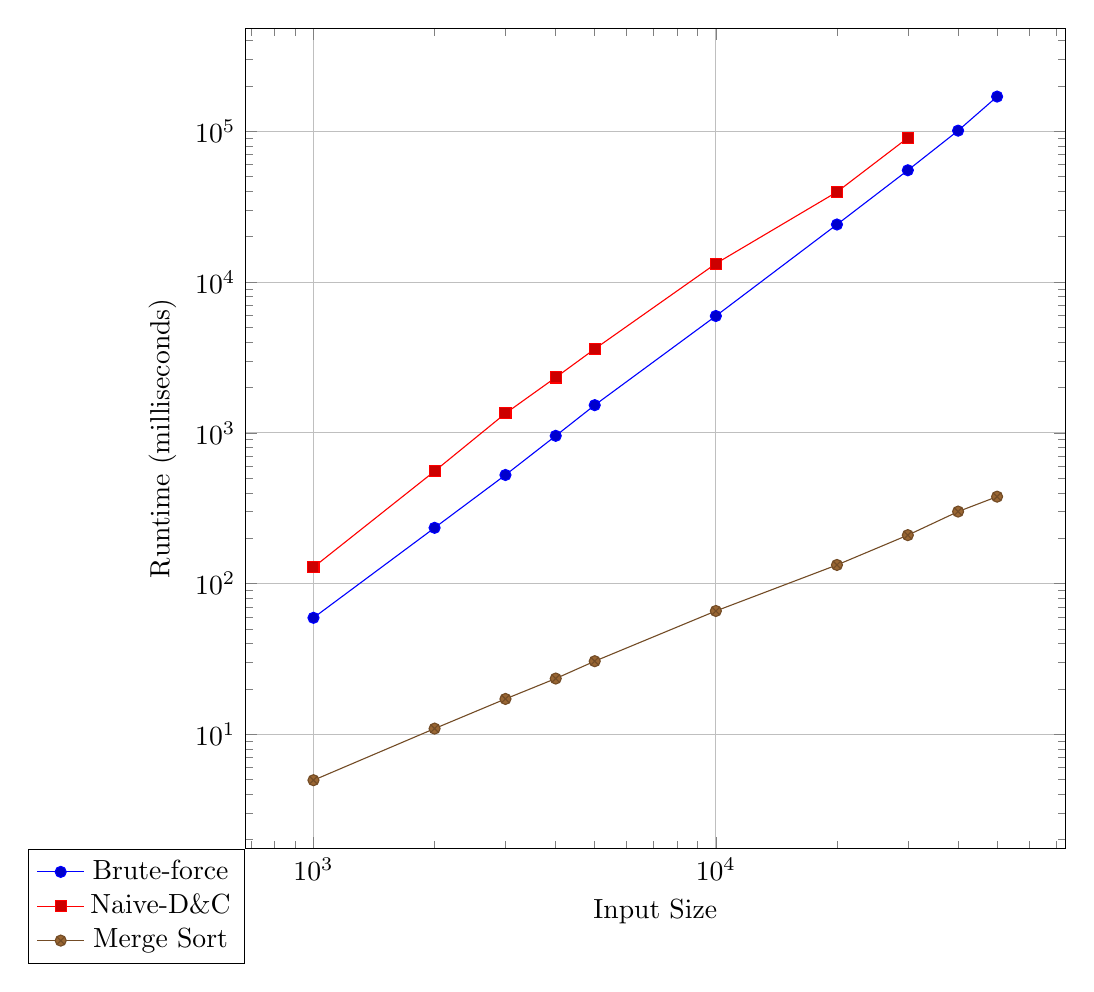
\begin{tikzpicture}
    \begin{loglogaxis} [
        legend style={at={(0,0)}, anchor=north east},
        grid=major,
        height=12cm,
        width=12cm,
        xlabel=Input Size,
        ylabel=Runtime (milliseconds),
    ]

    \addplot coordinates {
		(1000,59.2739344)
		(2000,234.2832087)
		(3000,525.2183437)
		(4000,955.0010203)
		(5000,1525.9585143)
		(10000,5955.0528526)
		(20000,24087.9588125)
		(30000,55162.801957)
		(40000,101022.8396414)
		(50000,169974.0216493)
		};
    \addlegendentry{Brute-force}

    \addplot coordinates {
		(1000,128.2862187)
		(2000,556.4429044)
		(3000,1345.2136756)
		(4000,2329.3997287)
		(5000,3598.7318755)
		(10000,13253.6118507)
		(20000,39603.0793427)
		(30000,90525.0232697)
		};
    \addlegendentry{Naive-D\&C}

    \addplot coordinates {
		(1000,4.9610378)
		(2000,10.913396)
		(3000,17.1679259)
		(4000,23.4416485)
		(5000,30.5465222)
		(10000,65.7936095)
		(20000,132.8696729)
		(30000,209.5165967)
		(40000,300.2828122)
		(50000,377.2132396)
		};
    \addlegendentry{Merge Sort}

    \end{loglogaxis}
\end{tikzpicture}

\paragraph{Slope of Lines}
\begin{itemize}
    \item Brute-force: 2
    \item Naive-D\&C: 2
    \item Merge Sort: 1
\end{itemize}

The largest input size the Brute-force method could solve in an hour is
roughly $10^7$.

\end{document}
